\documentclass{standalone}
\usepackage{tikz}
\usepackage{verbatim}
\usetikzlibrary{positioning}
\begin{document}
\pagestyle{empty}
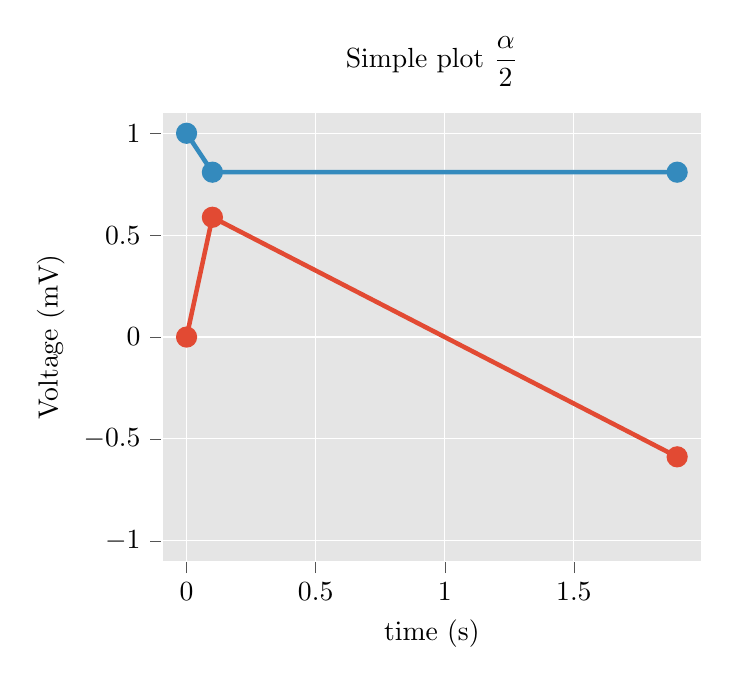
\begin{tikzpicture}

\definecolor{color0}{rgb}{0.886274509803922,0.290196078431373,0.2}
\definecolor{color1}{rgb}{0.203921568627451,0.541176470588235,0.741176470588235}

\begin{axis}[
axis background/.style={fill=white!89.8039215686275!black},
axis line style={white},
tick align=outside,
tick pos=left,
title={Simple plot \(\displaystyle \frac{\alpha}{2}\)},
x grid style={white},
xlabel={time (s)},
xmajorgrids,
xmin=-0.095, xmax=1.995,
xtick style={color=white!33.3333333333333!black},
y grid style={white},
ylabel={Voltage (mV)},
ymajorgrids,
ymin=-1.1, ymax=1.1,
ytick style={color=white!33.3333333333333!black}
]
\addplot [line width=1.64pt, color0, mark=*, mark size=3, mark options={solid}]
table {%
0 0
0.1 0.587785252292473
% [...]
1.9 -0.587785252292473
};
\addplot [line width=1.64pt, color1, mark=*, mark size=3, mark options={solid}]
table {%
0 1
0.1 0.809016994374947
% [...]
1.9 0.809016994374947
};
\end{axis}

\end{tikzpicture}
\end{document}